\documentclass[11pt,a4paper]{article}
\usepackage{amssymb}
\usepackage{amsthm}
\usepackage{amstext}
\usepackage{amsmath}
\usepackage{amsfonts}
\usepackage{verbatim}
\usepackage{geometry}
\usepackage{latexsym}
\usepackage{t1enc}
\usepackage{graphicx}
\usepackage[all]{xy}
\usepackage{makeidx}
\usepackage{slashed}
\usepackage{graphicx}
\usepackage{grffile}
\newtheorem{thm}{Theorem}[section]
\newtheorem{lem}[thm]{Lemma}
\newtheorem{cor}[thm]{Corollary}
\newtheorem{prop}[thm]{Proposition}
\DeclareMathOperator{\Tr}{Tr} \DeclareMathOperator{\comma}{,}

\numberwithin{equation}{section}

\geometry{left=2.5cm, right=2.5cm, top=2.5cm, bottom=2.5cm}

\linespread{1.1}

\frenchspacing

\begin{document}

\section{Part 1}

I have implemented my solution as a multi-modal classifier,
chosen as a boosted tree model (LightGBM) to avoid overfitting
on a relatively small dataset of $\sim$10,000 observations (OCR-scanned bounding boxes).

My repo consists of the following files,
\begin{itemize}
\item \texttt{data\_extraction.py}: This scripts loads the JSON files and creates
Pandas dataframes with each entry corresponding to a bounding box.
The train and test set dataframes are stored as Parquet files.

\item \texttt{feature\_engineering.py}: Here we preprocess the data to create
useful features for the model. There are four types of features:

1. \emph{Node height.} We observe that the ``linking'' entries define
a \emph{directed graph} in which the node heights $n_h=0,1,2$ correspond to
the classes Answer, Question and Header. (Presumably, the linking was obtained from
the spatial relationships of the bounding boxes.) As the graph information
is spread across multiple rows, we embed all nodes in a global graph
(one per \texttt{page\_id}) and compute the node height.

2. \emph{Layout information on bounding boxes.} Information on width, height,
center coordinates, aspect ratio and area of the bounding boxes.

3. \emph{Word embedding vectors of the text in the bounding boxes.}
We encode the text as word embedding vectors using the text embedding model
BAAI/bge-base-en-v1.5 available from Hugging Face.
We prepend the strings with the phrase ``Represent this document bounding box text for layout classification: ''
to make use of the model's context-aware embedding.

This step represents the words as 768-dimensional vectors. To avoid having the embedding vectors
take up the majority of the features and have the boosted tree do all its splits
on word embedding directions alone, we pipe the embedding vectors
into a 32-dimensional PCA. (The dimension 32 is observed downstream to yield
a better model than 16 or 24 dimensions.)

4. \emph{Ad-hoc punctuation features.} I expect words that contain ``?''
or ``:'' are Questions. Words of the form ``02/07/2023'', or words that contain currency symbols
or a high fraction of numerical characters are likely to be Answers.

\item \texttt{model.py}. We split the training dataset into a proper training training
set use to train our classifier. We set aside a validation set for hyperparameter tuning
(done with Optuna).

The model has a classification accuracy of 87\%. The confusion matrix and feature importance is shown below.

Some preliminary error analysis is done at the bottom of the script.

\begin{figure}[htbp]
    \centering
    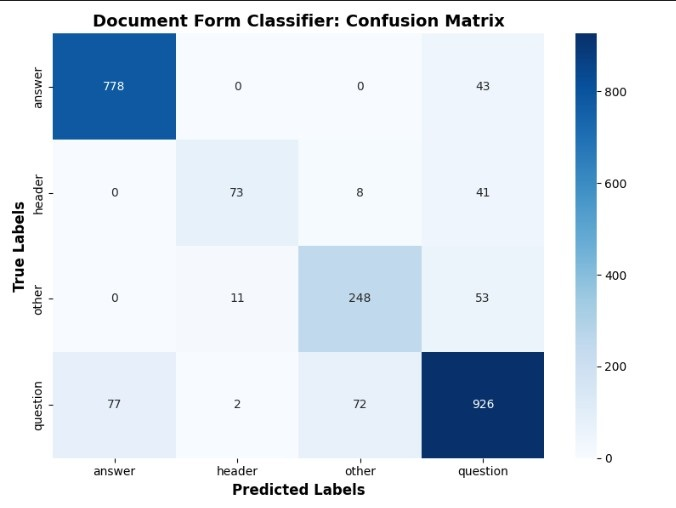
\includegraphics[width=0.7\textwidth]{confusion_matrix.jpg}
    \caption{Confusion matrix}
    \label{fig:stacked_image1}

    \vspace{1.5cm} % Adds vertical space between the images

    \includegraphics[width=0.7\textwidth]{feature_importance.jpg}
    \caption{Feature importance, based on number many times a feature
    is used to split data across all trees.}
    \label{fig:stacked_image2}
\end{figure}
\end{itemize}



\clearpage

\section{Part 2: Paper Club}

I would like to discuss \texttt{https://arxiv.org/pdf/2506.07972},
``HeuriGym: An Agentic Benchmark for LLM-Crafted Heuristics in
Combinatorial Optimization'' (ICLR 2026). The code is available on GitHub,

\noindent \texttt{https://github.com/cornell-zhang/heurigym}

The paper looks interesting because it offers a simple way
for LLMs to uncover heuristic algorithms for combinatorial optimization.
HeuriGym also allows automated improvement of existing heuristic algorithms
rather than manual tuning, thereby potentially shortening development
cycles considerably. The problems that could be addressed with this framework
are vehicle routing, pickup and delivery with time windows etc.

With this application in mind, the paper can be viewed as describing
Agentic LLMs that solve logistics problems.

HeuriGym can be used to generate solutions to the Pickup and Delivery with Time Windows 
problem as follows
\begin{enumerate}
\item Set up access to an LLM API (e.g., I used gemini-2.5-flash-lite). 
Then run \texttt{llm\_solver\_agent.py}. This will copy the following files from 

the \texttt{pickup\_delivery\_time\_windows} subfolder:
- \texttt{evaluator.py}
- \texttt{feedback.py}
- \texttt{main.py}
- \texttt{run.py}
- \texttt{solver.py} (ONLY FILE TO BE MODIFIED BY THE LLM)
- \texttt{utils.py}
- \texttt{verifier.py}

\item The new generated \texttt{solver.py} (generated from a prompt constructed 
from the input of the remaining files) can now be run on the data.
This consists of 30 .pdptw (Pickup and Delivery Problem with Time Windows) files.

\item The results of the generated routes are stored in the repo folder \texttt{heurigym/visualization\_outputs}

\begin{figure}[htbp]
    \centering
    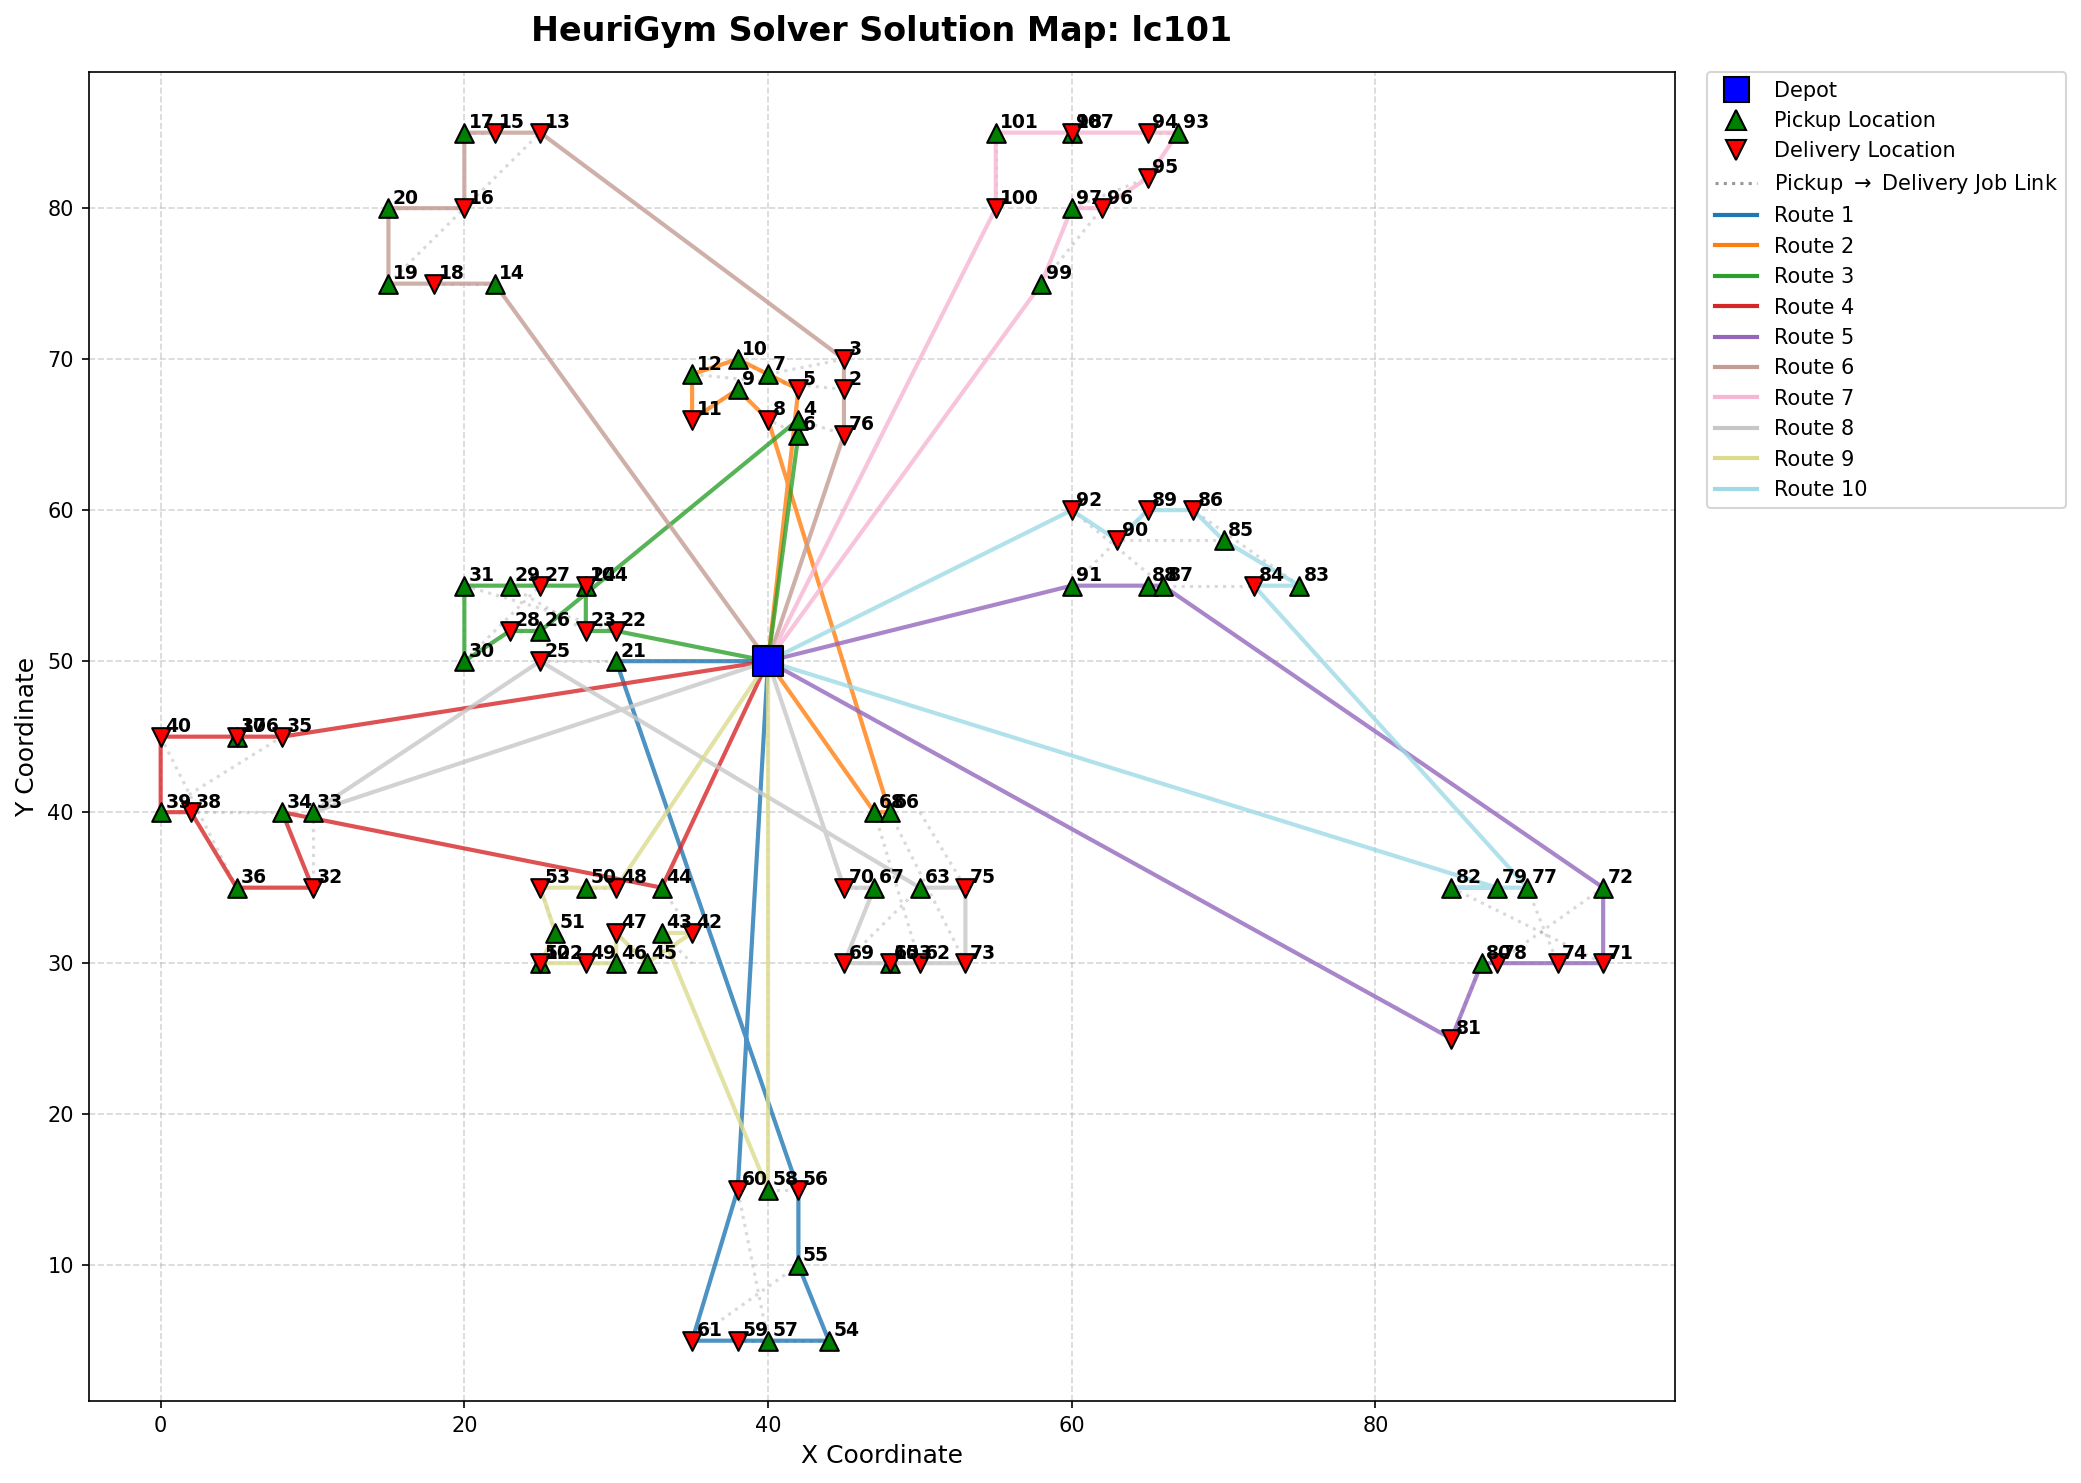
\includegraphics[width=1.0\textwidth]{lc101_route_map.png}
    \caption{Example output of Pickup and Delivery routes generated with HeuriGym}
    \label{fig:stacked_image3}
\end{figure}

\item The costs produced by the human expert vs. LLM generated routes are stored in
the repo folder \texttt{heurigym} as
\texttt{human\_expert\_baseline.json} and \texttt{heurigym\_cost\_results.json} respectively.
\end{enumerate}


\clearpage

\section{Part 3: Research Case - Case 2}

Given that OCR of the documents is available, I would go with Option 1.

Concretely, I would

\begin{enumerate}

\item Preprocess the OCR input with Recursive XY-Cut: separate the document
into bounding boxes by projecting first onto the X-axis, then onto the Y-axis,
splitting at the widest gap. Iterate until there are no gaps larger than a given threshold value.

\item Due to varying document resolution, scale all bounding box coordinates to
a fixed integer scale between 0 and 1000. For example, letting $(W, H)$ denote the width and height in pixels,
\begin{align}
x_\mathrm{normalized} &= \left\lfloor \frac{x_\mathrm{OCR}}{W} \times 1000 \right\rfloor \,, \\[2mm]
y_\mathrm{normalized} &= \left\lfloor \frac{y_\mathrm{OCR}}{H} \times 1000 \right\rfloor \,.
\end{align}
We choose integers to limit token usage and make the input predictable for the LLM's
vocabulary.

\item Interleave preprocessed bounding box data with OCR text in XML format
(to limit formatting overhead, so as to save token).

Our input may look like
\texttt{<block bbox="120,450,140,580">Invoice Number:</block>}

\texttt{<block bbox="120,590,140,710">INV-2026-89</block>}


\item Because the LLM is uni-modal, it doesn't understand spatial layout.
To ensure the LLM doesn't hallucinate new coordinates for the bounding boxes,
we demand that the LLM output a) must be JSON format, and b) the value of ``bbox''
in the JSON must be an array of 4 integer which match the coordinates inside
the \texttt{<block bbox ...} in the input XML.

In practice, we can do this by blocking invalid tokens at inference. We can
implement this with a Pydantic schema.



\end{enumerate}


\vspace{8mm}

\noindent Best Regards,

\noindent Kasper Jens Larsen

\end{document} 